\section{Auswertung}
    \subsection{Kenngrößen des Beheizbaren Ringkern}
        Zunächst wurde für die Beheizbare Spule mit Ringkern bei Raumtemperatur für verschiedenen Stromstärken je eine Hysteresenkurve
        aufgenommen um daraus anschließend die Remanenz-, Koerzitivfeldstärke und Maximale Magnetisierung zu bestimmen.\\
        Um die aufgenommen Spannungen der Gleichrichter verwenden zu können mussten diese zunächst in die Entsprechenden Magnetfeldstärken sowie Magnetisierungen umgerechnet werden.
        Für das Magnetfeld einer Spule gilt
        \begin{equation}
            H = \frac{n}{2\pi r}\frac{I_m}{U_m}U
        \end{equation}
        und nach Formel 2.5 aus der Anleitung für die Magnetisierung
        \begin{equation}
            M = \frac{U}{47\cdot 4\cdot \nu n_s q \mu_0}
        \end{equation}
        Mit $\nu = 50Hz$.\\
        Anschließend konnten die Kenngrößen aus folgenden Graphen abgelesen werden
        \begin{figure}[H]
            \centering
            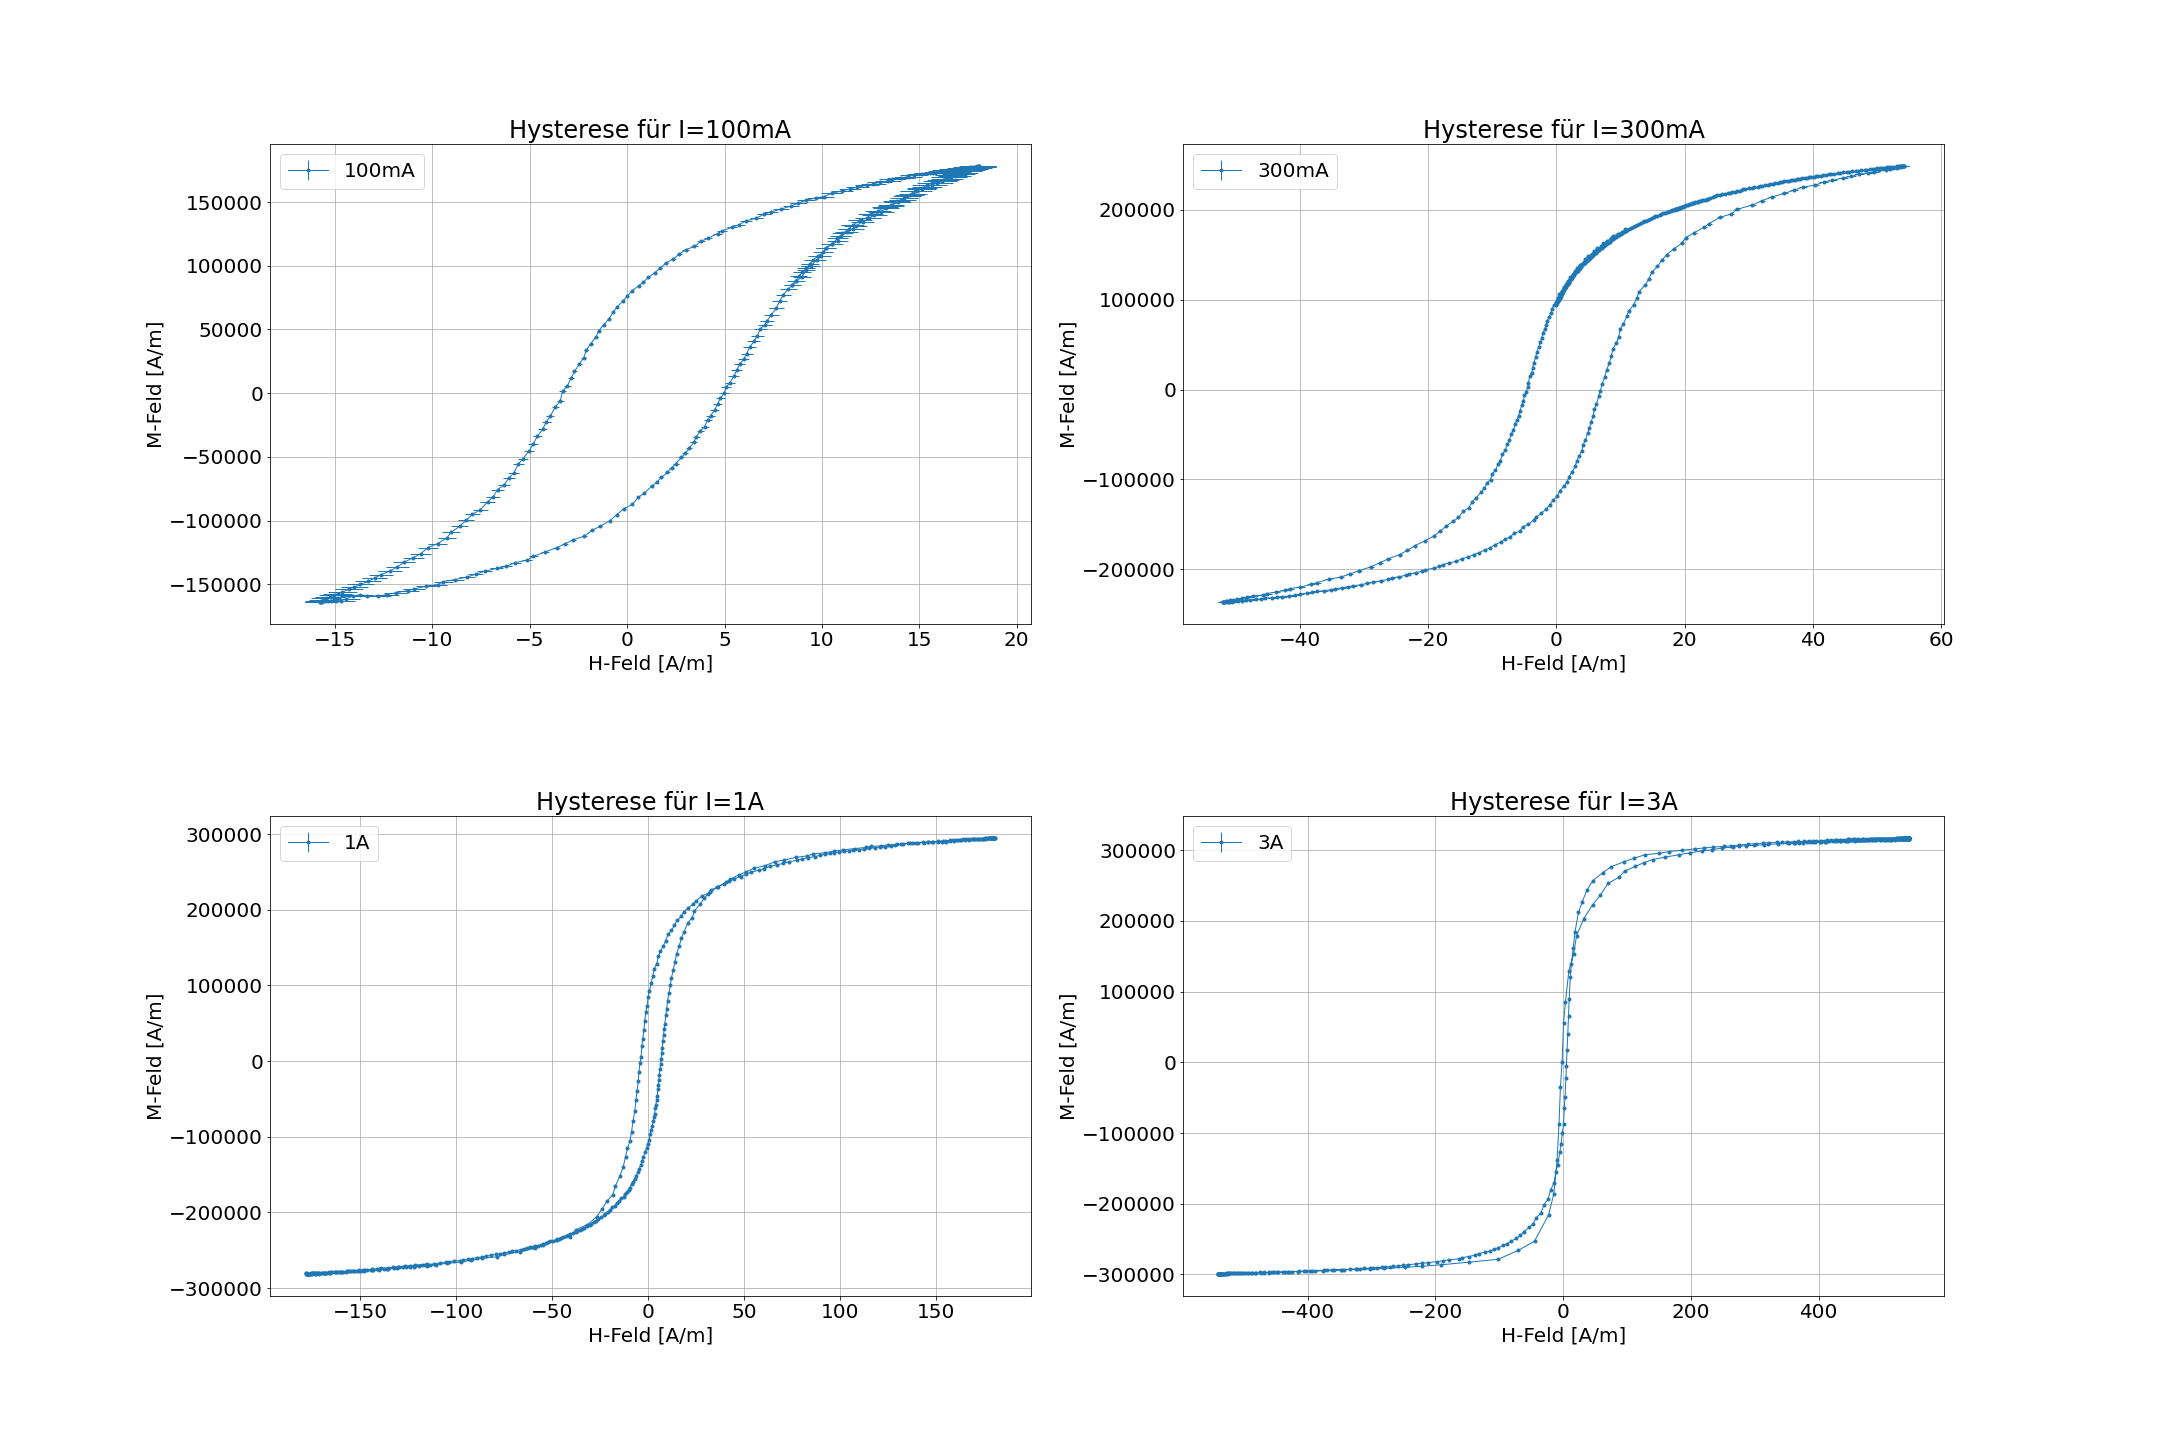
\includegraphics[width=\textwidth]{Images/Teil1.PNG}
            \label{Hysteresen}
            \caption{Hysteresenkurven bei Stromstärken 100mA,300mA,1A und 3A}
        \end{figure}
        Daraus lies sich folgende Tabelle zusammenstellen
        \begin{table}[H]
            \centering
            \begin{tabular}[]{c|c|c|c}
                Stromstärke & Remanenzfeldstärke [A/m] & Koerzitivfeldstärke [A/m] & maximale Magnetisierung [A/m] \\
                \hline
                100mA & 8.36e4 & 8.3 & 17.12e4 \\
                300mA & 10.66e4 & 11.33 & 24.26e4 \\
                1A    & 9.5e4 & 10.99 & 28.84e4 \\
                3A    & 7.15e4 & 6.86 & 30.86e4 \\
            \end{tabular}
            \caption{Kenngrößen des beheizbaren Ringkern bei Raumtemperatur}
        \end{table}
        Im allgemeinen entspricht die Tabelle unseren qualitativen Erwartungen, die maximale Magnetisierung steigt mit steigender Stromstärke und sowohl Remanenzfeldstärke als auch Koerzitivfeldstärke bleiben in etwa konstant. Die Fluktuation von sowohl Remanenzfeldstärke als auch Koerzitivfeldstärke
        wirkt hier jedoch fehl am platz, da diese nicht von der Stromstärke abhängen, was eine Messungenauigkeit impliziert.
    \subsection{Kommutierungskurve und Suszeptibilität}
        Um die Suszeptibilität des Systems zu bestimmen wurde durch die Variation des Primärspulenstroms jeweils eine Kommutierungskurve für 1 bis 0 A und 3 bis 0 A aufgenommen.
        Durch fitten des Models 
        \begin{equation}
            M(H) = A \cdot exp(-\frac{b}{H} + c) + d
        \end{equation}
        wurden zwei differenzierbare Äquivalente der aufgenommen Messdaten erzeugt um anschließend die Suszeptibilität in Abhängigkeit des angelegten Magnetfeldes zu plotten.
        \begin{figure}[H]
            \centering
            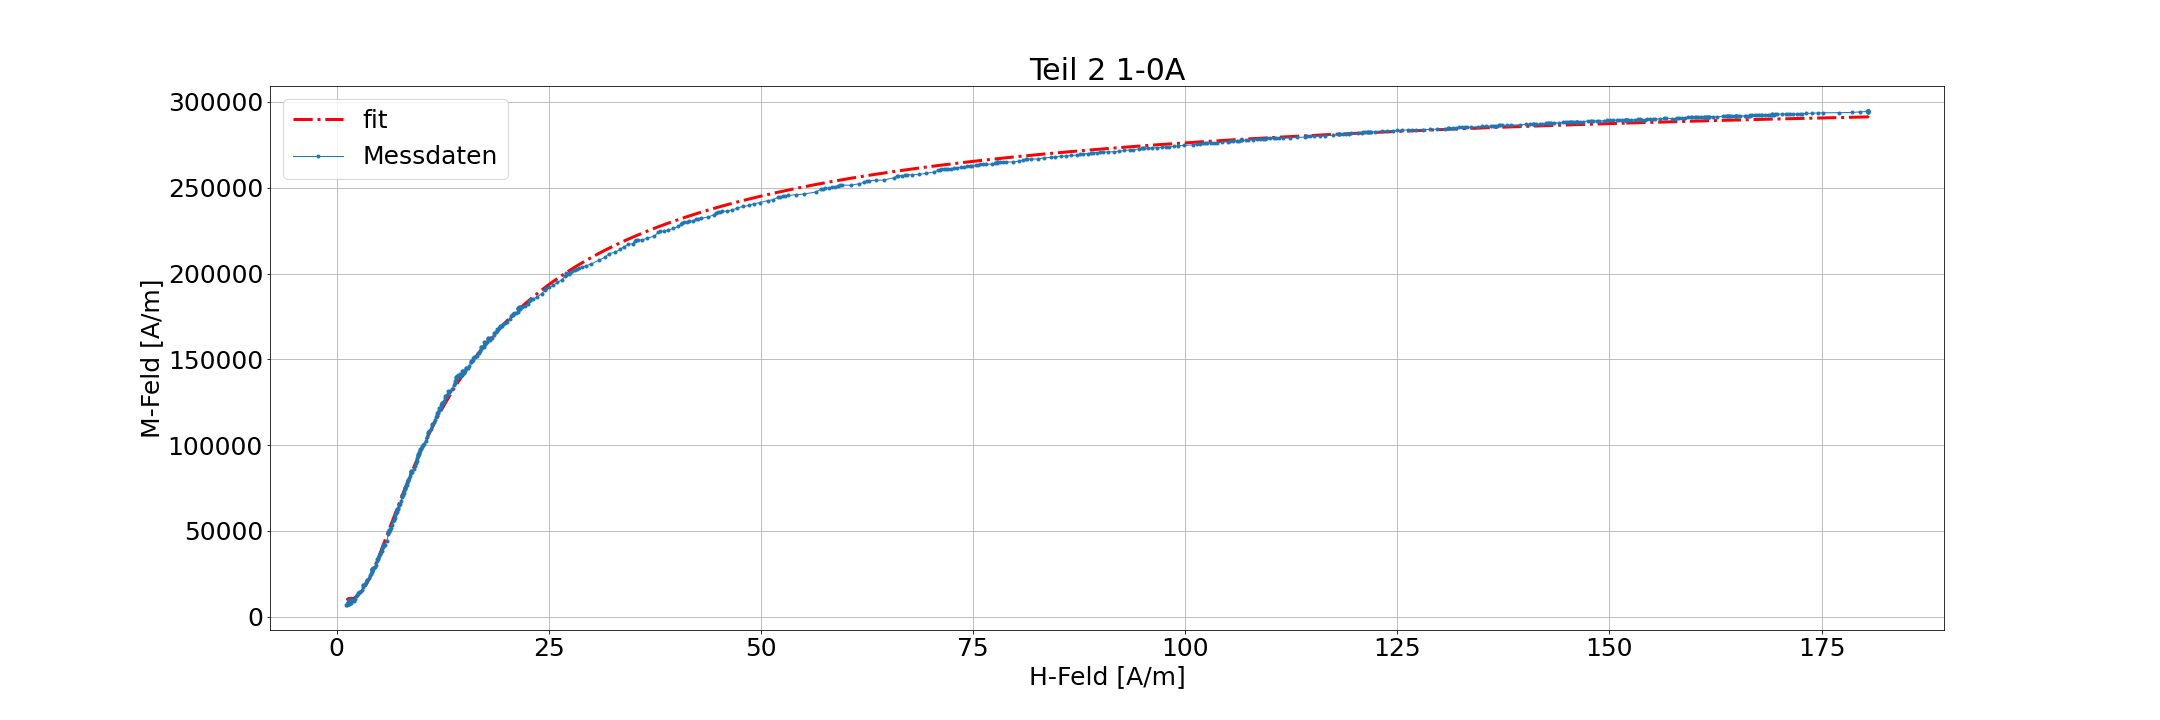
\includegraphics[width=\textwidth]{Images/Teil2Teil 2 1-0A.png}
            \label{Teil2-1A}
            \caption{Fit der Kommutierungskurve für 1 bis 0A}
        \end{figure}
        \begin{figure}[H]
            \centering
            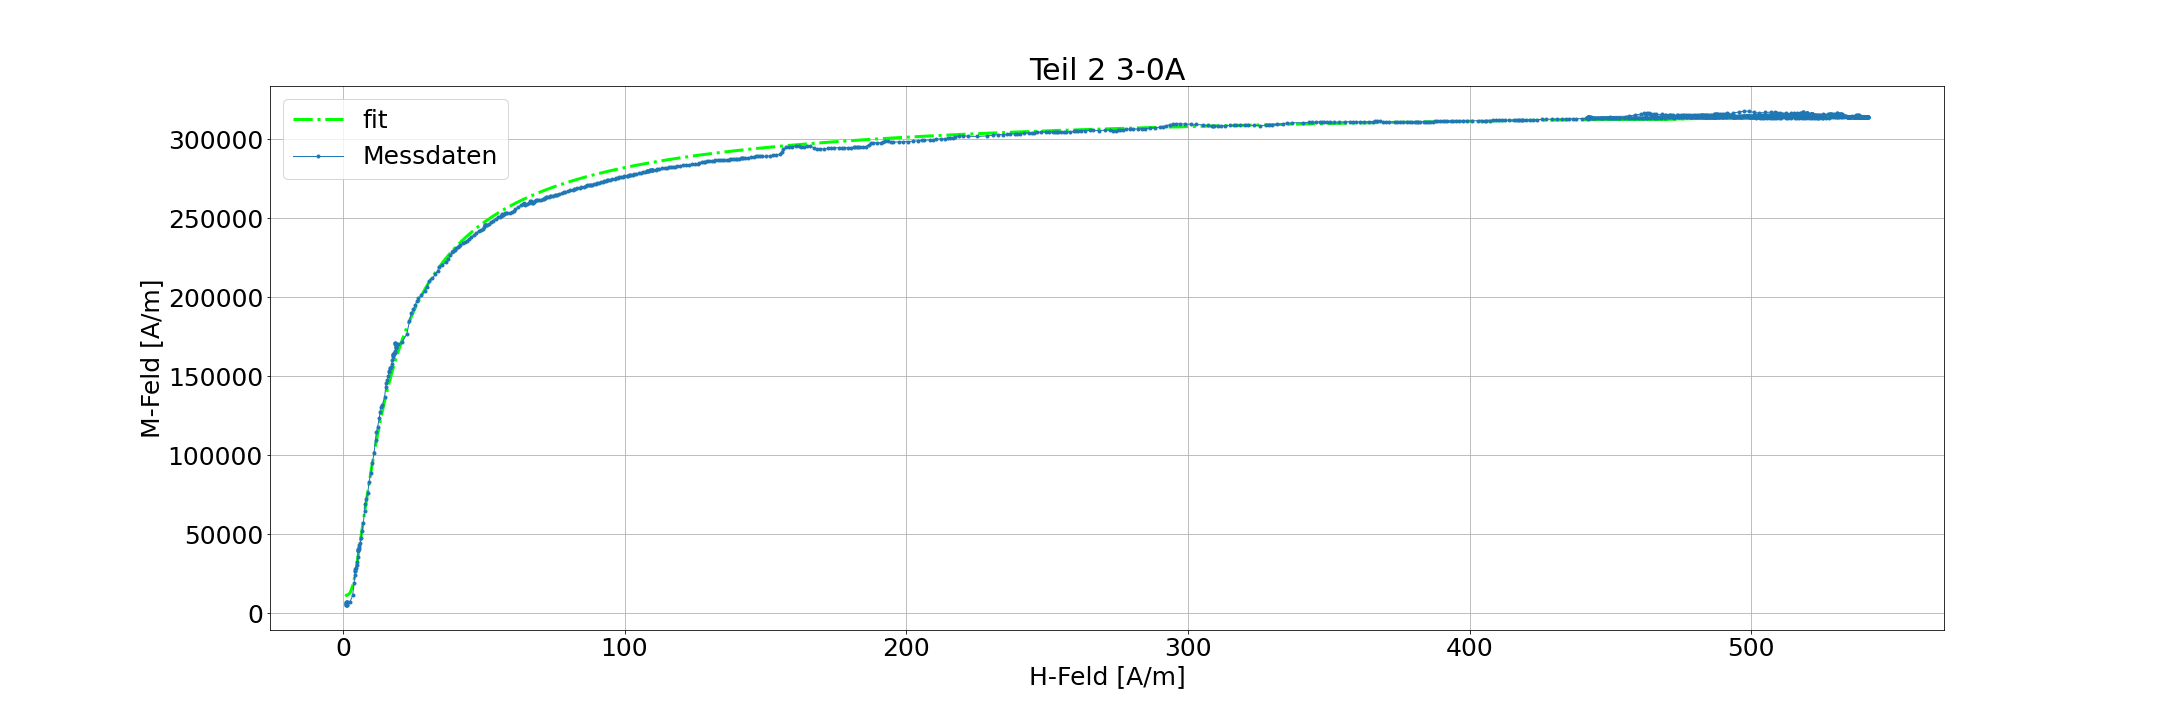
\includegraphics[width=\textwidth]{Images/Teil2Teil 2 3-0A.png}
            \label{Teil2-3A}
            \caption{Fit der Kommutierungskurve für 3 bis 0A}
        \end{figure}
        \begin{figure}[H]
            \centering
            \includegraphics[width=\textwidth]{Images/Teil2Differentielle Suszeptibilität.png}
            \label{DiffSus}
            \caption{Plot der Suszeptibilität für beide Kommutierungskurven}
        \end{figure}
            Der Verlauf der differentiellen Suszeptibilität ist für beide Kurven physikalisch sinnvoll, da für beide Kurven ein Verlauf proportional zu $\frac{1}{H}$ zu erkennen ist ($\chi \propto \frac{1}{H}$). Auch ist zu erkennen,
            das für geringere Stromstärken die maximale Suszeptibilität abnimmt.
    \subsection{Temperaturabhängigkeit und Curie Temperatur}
        \begin{figure}[H]
            \centering
            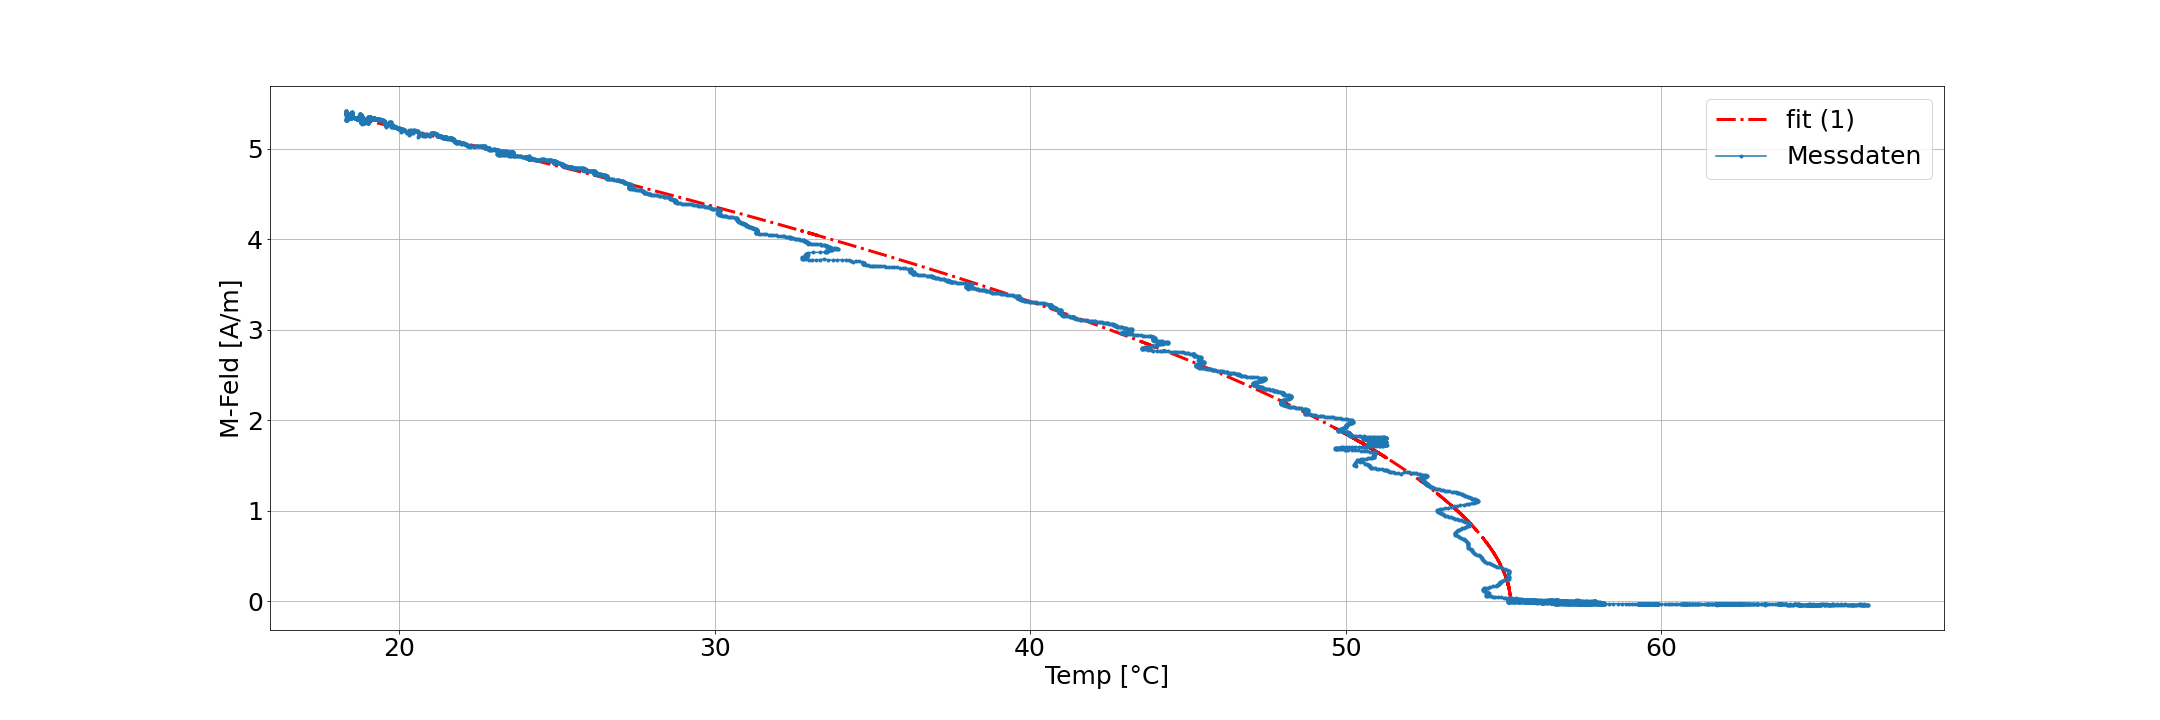
\includegraphics[width=\textwidth]{Images/Teil3.png}
            \label{Temp}
            \caption{Temperaturabhängigkeit der Magnetisierung}
        \end{figure}
        Bei Aufnahme der Temperaturabhängigkeit der Magnetisierung ist deutlich zu Erkennen, das bei Steigenden Temperaturen durch die zunehmende innere Energie
        auch die Unordnung der internen Dipole zunimmt und somit die Magnetisierung abnimmt. Bei ca. 55°C verfällt die Magnetisierung vollständig. Dort ist die Curie-Temperatur erreicht.
        $$T_C  = (55 \pm 2)°C$$
    \subsection{Ringkern mit Spalt}
        Für den Ringkern mit Spalt wurde zunächst analog zum ersten Teil der Auswertung eine Hysteresenkurve aufgenommen als Referenz für die folgenden Messungen mit Variablen Spaltbreiten.
        Aus der Analyse des Graphen ergab sich
        \begin{figure}[H]
            \centering
            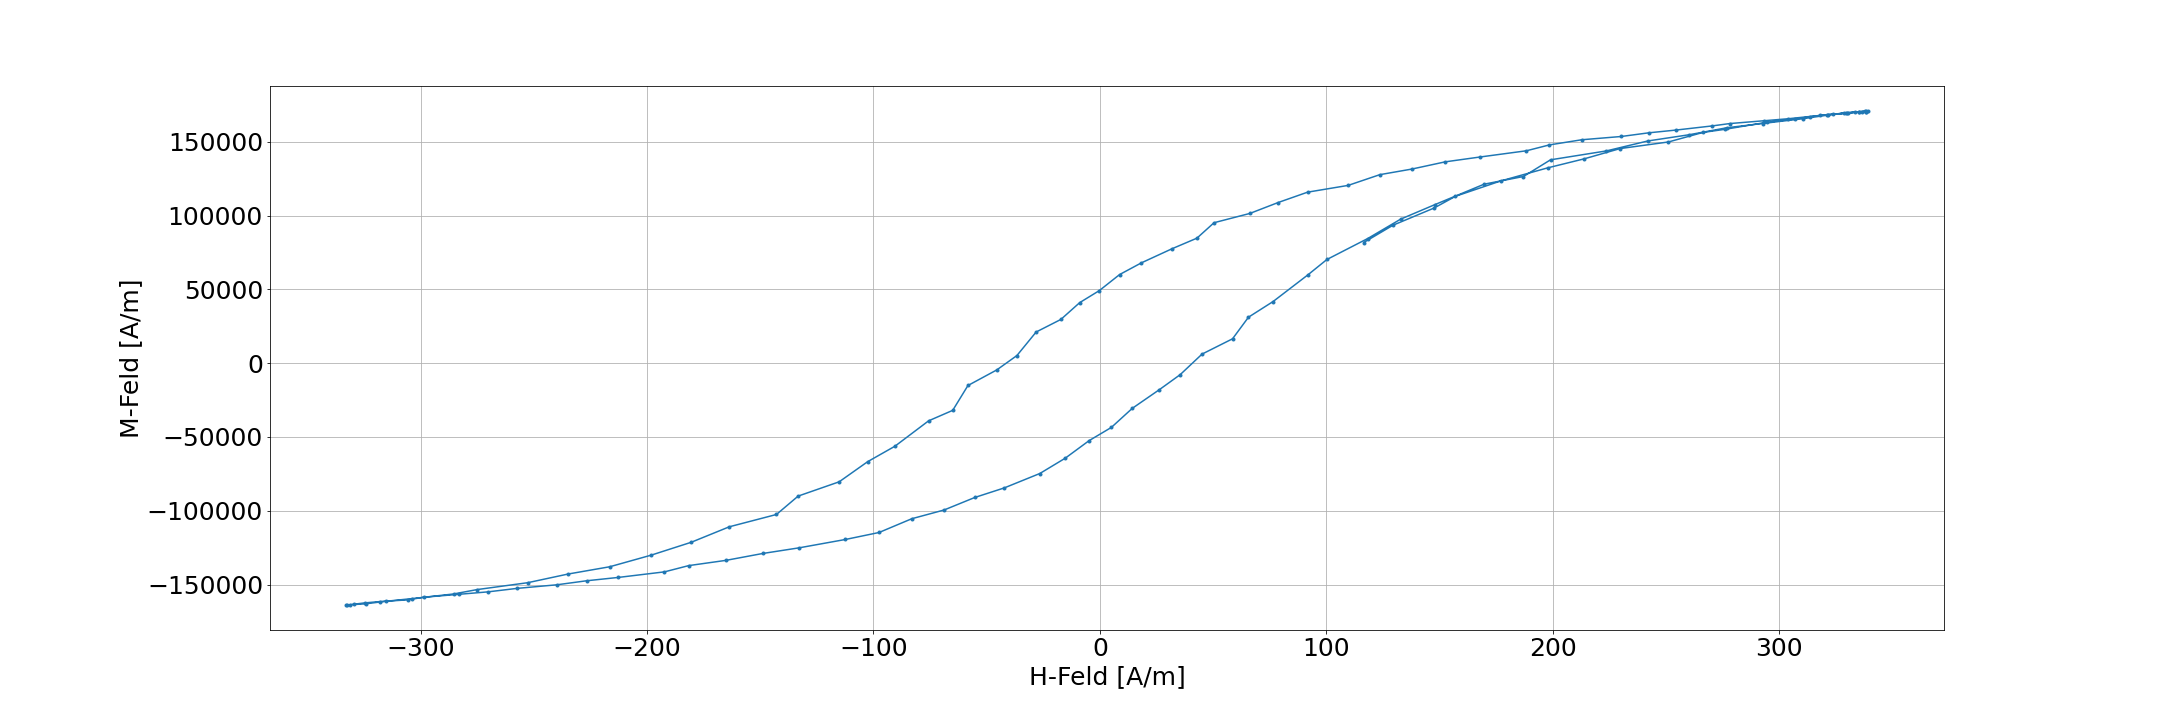
\includegraphics[width=\textwidth]{Images/Teil4.1.png}
            \label{Hyst4}
            \caption{Hysteresenkurve für den Ringkern mit Spalt bei 0.94A}
        \end{figure}
        Um nun anschließend den Entmagnetisierungsfaktor N als Funktion der Spaltbreite zu ermitteln wurden Hysteresenkurve bei verschiedenen Spaltbreiten und gleicher Maximalen Magnetisierung
        aufgenommen.